\subsection{Overview}
\label{principles-overview}

% ------------------------------------------------------------------------------

\subsubsection{Taxonomy}
\label{taxonomy}

After the goal of manifold learning has been formalized, it shall now be laid 
out how the problem is approached by LLE as the conceptual parent of SSLLE 
(the incorporation of prior information is a rather different matter that will 
be addressed in chapter \ref{sslle}; apart from this, the basic functionalities 
of SSLLE and LLE are identical and will therefore be presented as one). 
Much of the theoretical foundation for LLE has been discussed only in later 
work.
In order to provide a more integrated background, explanations will therefore be 
given in a broader context of local graph-based manifold learning (LGML), which 
also comprises LEM and HLLE.
The particular relationship of the three methods shall be made clear along the 
way.

LGML arises from a variety of geometric 
intuitions and computational implementations.
Nonetheless, methods share common structures that allow for interpretation in a 
more abstract framework (\citet{bengioetal2003}, \citet{bengioetal2004}).
It should be noted that such a framework might be established from several 
angles; after all, the different approaches attempt to solve the same problem 
and can thus be translated into one another in various ways.

Figure \ref{fig-models-overview} depicts a schematic overview on the models 
studied here, representing the specific perspective taken within this report.
All of these belong to the realm of \textit{spectral} models.
The non-spectral group includes, among others, techniques based on neural 
networks and is not discussed here \citep{vandermaatenetal2009}.

\begin{figure}[H]
    \centering
    % https://docs.google.com/drawings/d/1982RyrkrJzhR-LHvR3xUmuCMEdpiK8qkm00HBvKMY9I/edit
    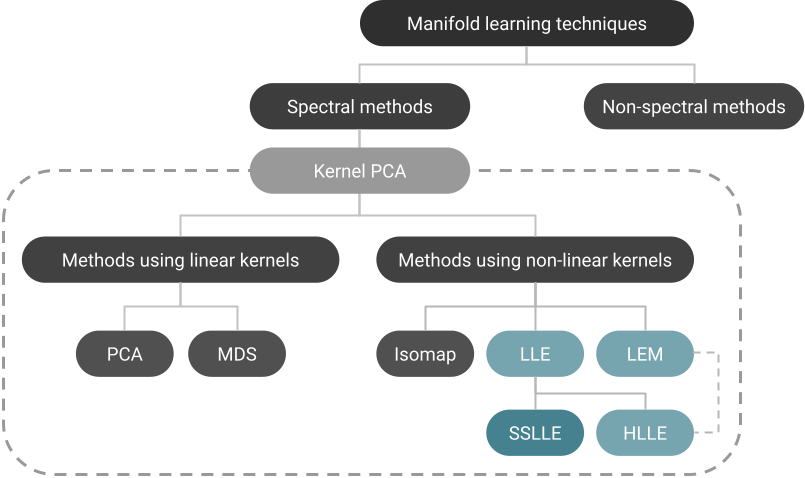
\includegraphics[trim = 0 0 0 0, clip, % left bottom right top
      width = \textwidth]{figures/models_overview}
    \caption[Overview on selected manifold learning models]{A schematic overview 
    on selected methods of manifold learning (the list is by no means extensive 
    and could arguably be ordered in several alternative ways). 
    \textit{Source:} own representation, inspired by a similar example given in 
    \citet{vandermaatenetal2009} and re-interpreted with the findings in 
    \citet{bengioetal2004}.}
    \label{fig-models-overview}
  \end{figure}

% ------------------------------------------------------------------------------

\subsubsection{Intuition}
\label{intuition}

As indicated in figure \ref{fig-models-overview}, this report will 
sketch the idea behind LGML in the light of 
\textit{kernel principal component analysis (kernel PCA)}.
Kernel PCA was actually proposed first and later shown to link the other 
concepts by a unified idea (\citet{hametal2003}.
It makes for an appealing framework that provides a useful general 
intuition to manifold learning and subsumes the other methods in a 
way beneficial to the important task of out-of-sample extension \citep{bengioetal2004}.
\\

\textbf{Kernel PCA.} Kernel PCA builds upon two fundamental concepts 
in machine learning: it performs \textit{principal component analysis (PCA)} on 
data transformed by the \textit{kernel trick}.
It undertakes two subsequent steps.
First, features of interest are extracted from the data by kernelization. 
These are taken to capture the intrinsic data structure and may therefore be 
understood as an approximation to the latent manifold properties.
In the end, they constitute a matrix representation.
Second, PCA finds the principal axes along which these intrinsic properties 
vary, yielding the desired reduction in dimensionality by preserving the most 
relevant latent dimensions \citep{schoelkopfetal1998}.

\begin{itemize}

  \item[] \textbf{Kernelization.} By kernelization, mapping the data to a 
  space $\mathcal{F}$ of arbitrarily high dimension, features may be obtained 
  that relate to the input in a non-trivial way\footnote{
  Support vector machines use the kernel trick to achieve linear separability. 
  An intuitive example may be given by data observed in two classes that form 
  concentric circles in $\R^2$. 
  While such data are not linearly separable in two dimensions, they are in three: 
  mapping the classes to different heights enables separation by a horizontal 
  hyperplane.
  This example also hints at the idea of (spectral) clustering to which kernel 
  PCA is indeed intimately related \citep{bengioetal2004}.
  }.
  Crucially, the feature map $\phi: \RD \rightarrow \mathcal{F}$ need not be 
  computed explicitly, which might prove prohibitively expensive.
  Kernelization instead solely relies on inner products $\langle \phi(\x_i), 
  \phi(\x_j) \rangle$ of the transformed inputs.
  Employing Mercer's theorem of functional analysis, these inner products may 
  be interpreted as performed by a continuous kernel 
  % Remove domain and co-domain of kappa, might be wrong, needs the Hilbert 
  % space after all, right
  $\kappa(\x_i, \x_j)$ in some space with Hilbert property.
  Appropriate choice of $\kappa$ then allows for the data to be represented by a 
  matrix $\K \in \R^{N \times N}, \K_{ij} = \kappa(\x_i, \x_j)$.
  This matrix is the numerical data representation derived with respect to their 
  latent properties. \citep{schoelkopfetal1998}.
  Precisely how it is computed depends on the choice of the kernel function 
  $\kappa$ and gives rise to different techniques \citep{hametal2003}.
  
  \item[] \textbf{PCA.} PCA is a quite powerful technique by itself.
  It finds the directions of maximum variance through eigenanalysis of the 
  empirical covariance matrix, yielding the most important axes of inter-feature 
  relations that coincide with the principal eigenvectors of the covariance 
  matrix.
  The data are projected into the linear subspace spanned by these $d$ 
  eigenvectors, thereby mapping the observations to a coordinate system given 
  by the linear feature combinations that represent the strongest 
  (co)variability.
  Note that for this transformation to actually rotate the coordinate system 
  about the origin, the data must be mean-centered beforehand.
  PCA thus performs an orthogonal input transformation that allows for 
  dimensionality reduction at minimal information loss \citep{cayton2005}.
  In kernel PCA, this eigenanalysis is implicitly performed in the feature space 
  $\mathcal{F}$.
  Algorithmically, it boils down to diagonalizing the kernel matrix $\K$ 
  \citep{schoelkopfetal1998}.
 
\end{itemize}

Figure \ref{fig-spirals} visualizes the idea of kernel PCA.
The original data (\textit{left}) are observed in two dimensions but clearly 
intrinsically one-dimensional, where the non-linear manifold feature is 
expressed by coloring. 
The kernel trick creates a feature map, visualized here as a projection of 
the intrinsic feature to a third coordinate axis (\textit{middle}). 
Coercing the data to this dimension as the sole axis of variation yields the 
desired one-dimensional representation (\textit{right}). 

\begin{figure}[H]
 \centering
 \begin{subfigure}[c]{0.29\textwidth}
   \centering
   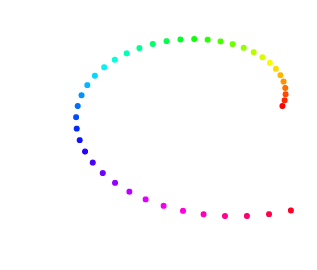
\includegraphics[%trim = 50 0 0 0, clip, % left bottom right top
   width = \textwidth]{figures/spirals-2d}
 \end{subfigure}
 \hfill
 \begin{subfigure}[c]{0.4\textwidth}
   \centering
   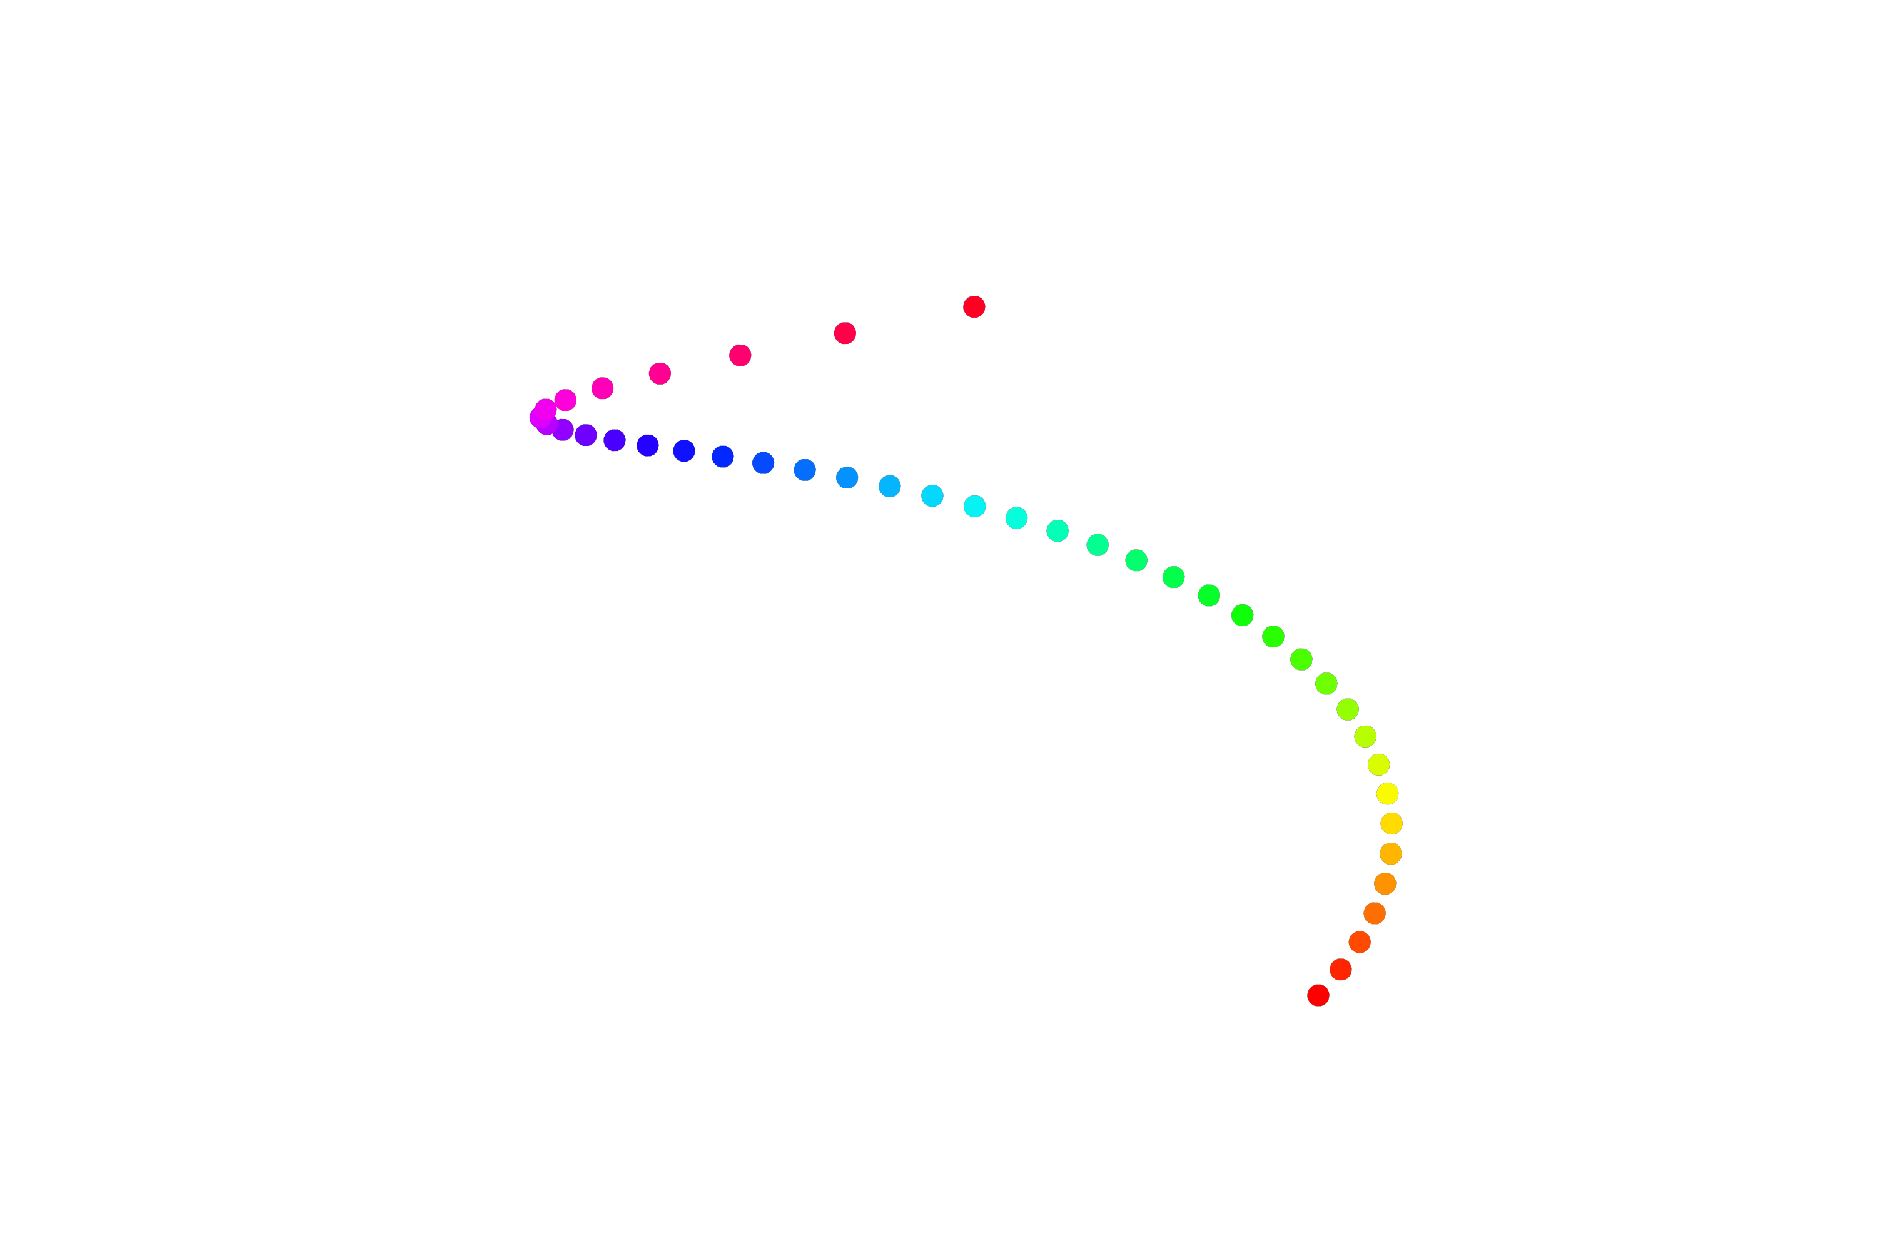
\includegraphics[%trim = 250 50 100 50, clip, % left bottom right top
   width = \textwidth]{figures/spirals-3d}
 \end{subfigure}
 \begin{subfigure}[c]{0.29\textwidth}
   \centering
   
\includegraphics[%trim = 0 0 0 300, clip, % left bottom right top
   width = \textwidth]{figures/spirals-1d}
 \end{subfigure}
  \caption[Schematic idea of kernel PCA]{Schematic idea of kernel PCA: from data
  observed in two dimensions, but clearly of intrinsic dimensionality one 
  (\textit{left}), create a mapping to a higher-dimensional feature space 
  (\textit{middle}), reduction of which to its principal axes yields the desired 
  one-dimensional representation (\textit{right}).
  \textit{Source:} own representation, using a subset of \texttt{mlbench}'s 
  noise-free \texttt{spirals} data. Note that this is but a schematic depiction 
  where the mid and right representation have not been created by an actual 
  implementation of kernel PCA.}
  \label{fig-spirals}
\end{figure}

% ------------------------------------------------------------------------------

\subsection{Conceptual Framework of LGML}
\label{framework}

% ------------------------------------------------------------------------------

\subsubsection{Motivation}
\label{motivation}

If kernel PCA sounds like a powerful concept, the crux of course lies in 
finding an appropriate kernel function.
The nature of the feature map applied to the input data determines the kind of 
mapping that may be learned and serves to distinguish the various techniques.
As foreshadowed in figure \ref{fig-models-overview}, spectral methods decompose 
into groups using \textit{linear} and \textit{non-linear} kernels, respectively.
This distinction directly translates to the feature map $\phi$.
Linear methods suffer from the confinement to finding linear subspaces \citep{vandermaatenetal2009}.
PCA in its standard form can be interpreted as kernel PCA by identifying the 
kernel function with the covariance function.
It thus returns the subspace of greatest variability in the original input 
features \citep{hametal2003}.
The closely related \textit{multi-dimensional scaling (MDS)} yields the 
same result\footnote{
At least, in its metric form; there are alternative formulations of MDS that 
are not equivalent to PCA (see, for example, \citet{williams2002}).
}, albeit from a different intuition \citep{sauletal2006}.

As extensively discussed above, $\X$ must often be 
assumed to lie on a non-linear manifold $\mani \subset \RD$, which is precisely 
why kernelization is usually performed such that the resulting feature space is 
related to the input space in a non-linear way \citep{schoelkopfetal1998}.
Conceivably, there is no obvious way to arrive at such a mapping.
\textit{Graph-based} models therefore approach the problem from an alternative 
angle.
In fact, they do not even perform kernelization explicitly: they transform the 
data in a way that can be shown to correspond to applying a (data-dependent) 
kernel function\footnote{
The report does not discuss the actual kernel function as their illustrative 
ability is considered rather limited.
For an explicit formulation of kernels in LLE, LEM and HLLE see for example \citet{bengioetal2004} and \citet{weinbergeretal2004}.
}, 
but the fundamental intuition is a different one. 
\\

\textbf{Non-linearity.} 
The key idea in graph-based learning is to approximate the manifold by a 
discretized graph representation.
Such a graph may be intuitively imagined as a skeletal model of $\mani$ (an 
example is given in \ref{fig-neighbor-graph}).
This way, distances may be measured along the approximated manifold 
surface rather than in the ambient Euclidean space, effectively enabling 
non-linearity.
Functionals that vary across methods are used to describe properties of the 
graph -- essentially a proxy of the latent manifold properties 
\citep{sauletal2006}.
\\

\textbf{Locality.} A second desideratum in general manifold learning is the 
ability to treat highly non-linear manifolds with sufficiently local focus.
Non-convexity means $\mani$ is isometric to a non-convex subset of Euclidean 
space \citep{donohogrimes2003}. 
Intuitively, such behavior requires careful tracing of the manifold surface.
LGML methods therefore focus on solely local manifold properties 
\citep{cayton2005}.
They are frequently contrasted to \textit{Isomap}, one of the 
earliest and most prominent examples of global manifold learning.
Isomap retains pairwise distances between points on the manifold surface as 
measured along graph edges via geodesic curves\footnote{
It is thus a non-linear variant of MDS, which uses standard Euclidean distances 
\citep{tenenbaumdesilvalangford2000}.
} \citep{tenenbaumdesilvalangford2000}.
Its central assumptions are global isometry and convexity of the parameter 
space \citep{tenenbaumdesilvalangford2000}.
While it yields good results in many applications, Isomap does not sufficiently 
account for the curvature of strongly non-convex manifolds.
In order to avoid this drawback, local methods limit isometry to only hold 
between neighboring points and relax the parameter space 
condition to open, connected subspaces \citep{donohogrimes2003}.
\\

\textbf{Algorithmic procedure.}
Summing up the above, LGML methods use functionals defined on graph 
approximations of the manifold to capture the intrinsic data structure.
This information is stored in a matrix representation $\M$ that is 
directly linked to the kernel matrix $\K$.
Eigenanalysis of $\M$ then leads to the sought-for low-dimensional subspace 
coordinates.

The resulting algorithmic pattern may be stated as follows 
\citep{bengioetal2003}:

\begin{tight_enumerate}
  \item Construct a neighborhood graph $\mathcal{G}$ from the observed data.
  \item Analyze the graph properties with an appropriate functional and derive 
  a matrix representation $\M$ thereof.
  \item Find the eigenvalues and associated eigenvectors of $\M$.
  \item From the principal (top or bottom) eigenvectors, as determined by the 
  ordered eigenvalues, retrieve the low-dimensional coordinates.
\end{tight_enumerate}

Figure \ref{fig-kpca-lgml} provides a final view on the LGML concept and its 
algorithmic operationalization in the kernel PCA context.

\begin{figure}[H]
  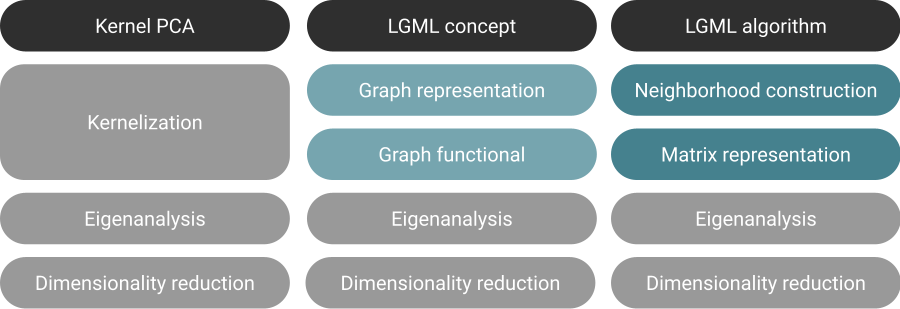
\includegraphics[%trim = 0 0 0 300, clip, % left bottom right top
  width = \textwidth]{figures/kpca_lgml_algo}
  \caption[Kernel PCA and LGML]{Conceptual view of LGML, interpreted as a form 
  of kernel PCA.
  \textit{Source:} own representation.}
  \label{fig-kpca-lgml}
\end{figure}

% ------------------------------------------------------------------------------

\subsubsection{Graph Approximation}
\label{graph}

All LGML methods fundamentally build on graph approximations of the 
manifold surface.
Note that these graphs are constructed from neighborhood relations in the 
high-dimensional observation space and do not require any prior information 
about the latent manifold coordinates.
\\

\textbf{Neighborhoods.} 
A neighborhood of $\x \in \X$ is a subset of $\X$ containing another, open 
subset of $\X$ of which $\x$ is an element.
Members of the neighborhood are called neighbors of $\x$.
In metric spaces neighborhoods are defined via distances and therefore 
translate to open balls around each point \citep{waldmann2014}.
This distance-based construction locally applies to manifolds as a direct 
consequence of their local isometry to the Euclidean observation space 
\citep{mafu2011}.
There are two principal ways to build a neighborhood around $\x \in \X$, 
both of which usually employ the squared Euclidean norm\footnote{
In principle, alternative metrics are applicable, for instance such 
that measure angles \citep{belkinniyogi2004}.
} $\| \cdot \|^2$.
Let $\mathcal{N}: \X \rightarrow \X^{\ell}, \x \mapsto \mathcal{N} (\x)$ be a 
constructor that assigns a set of neighbors to $\x$.
The first possibility is to restrict the size of the neighborhood to the $k$ 
points\footnote{
In presence of ties in pairwise distances k may vary across the data, but with 
zero probability in continuous feature spaces.
} with the smallest distance to $\x$, such that
$\ell = k$ and 

\begin{equation}
  \mathcal{N}_k(\x) = \{\x_j \in \X: \| \x - \x_j \|^2 \leq d_{(k)}\},
  \label{eq-kneighborhood}
\end{equation}

with $d_{(k)} \in \R$ being the $k$-th instance of ordered pairwise distances 
between $\x$ and all other points.
Alternatively, the neighborhood may be constructed by collecting all points that
have a maximum distance of $\epsilon \in \R$ to $\x$, yielding 

\begin{equation}
  \mathcal{N}_{\epsilon} (\x) = \{\x_j \in \X: \| \x - \x_j \|^2 \leq \epsilon\}
  \label{eq-epsneighborhood}
\end{equation}

and $\ell = |\mathcal{N}_{\epsilon} (\x)|$ \citep{heetal2005}.
\\

Both $k$ and $\epsilon$ are hyperparameters that must be specified up-front.
Their choice reflects beliefs about the topological structure of $\mani$ -- 
smaller neighborhoods corresponding to a higher degree of non-linearity -- and 
may affect performance rather strongly \citep{sudderth2002}.
Chapter \ref{challenges} will discuss this trade-off, which is also addressed in 
the practical implementation (section \ref{experiment}), in more detail.
In this, the remainder of the report will focus on the $k$-neighborhood notion 
as it is typically more easily specified due to its inherent scale invariance 
and has attracted rather more attention in general research\footnote{
Yet, \citet{tenenbaumdesilvalangford2000} note that, when local dimensionality 
is not constant across the observed data, $\epsilon$-neighborhoods might provide 
more reliable results.
}. 
\\

\textbf{Neighborhood graphs.}
$\mani$ can now be characterized by a \textit{neighborhood 
graph} $\mathcal{G} = (\mathcal{V}, \mathcal{E})$, still assuming it is 
sampled well by $\X$. 
Inputs $\x \in \X$ form vertices $\mathcal{V}$ and edges $\mathcal{E}$ 
indicate neighborhood relations \citep{belkinniyogi2001}.
Each vertex is connected to its $k$ nearest neighbors or all points 
within $\epsilon$-radius, depending on the neighborhood definition.

\begin{minipage}[b]{0.5\textwidth}
  It is easy to see that $k$-neighborhoods are an asymmetric notion; for one 
  point to be among another's $k$ nearest neighbors the reverse need not be 
  true.
  $k$-neighborhoods therefore lead to directed graphs.
  Conversely, the $\epsilon$-distance boundary holds in both directions and 
  produces undirected graphs \citep{heetal2005}.
  Figure \ref{fig-neighbor-graph} shows how a neighborhood graph may be used as 
  an approximation for the example of the S-curve manifold.
  It was built using $k$-neighborhoods with $k = 3$.
  For a densely sampled set of points, the graph representation should yield a 
  fairly good approximation of the manifold surface.
\end{minipage}
\begin{minipage}[b]{0.05\textwidth}
  \phantom{xxx}
\end{minipage}
\begin{minipage}[b]{0.45\textwidth}
  \begin{figure}[H]
    \centering
    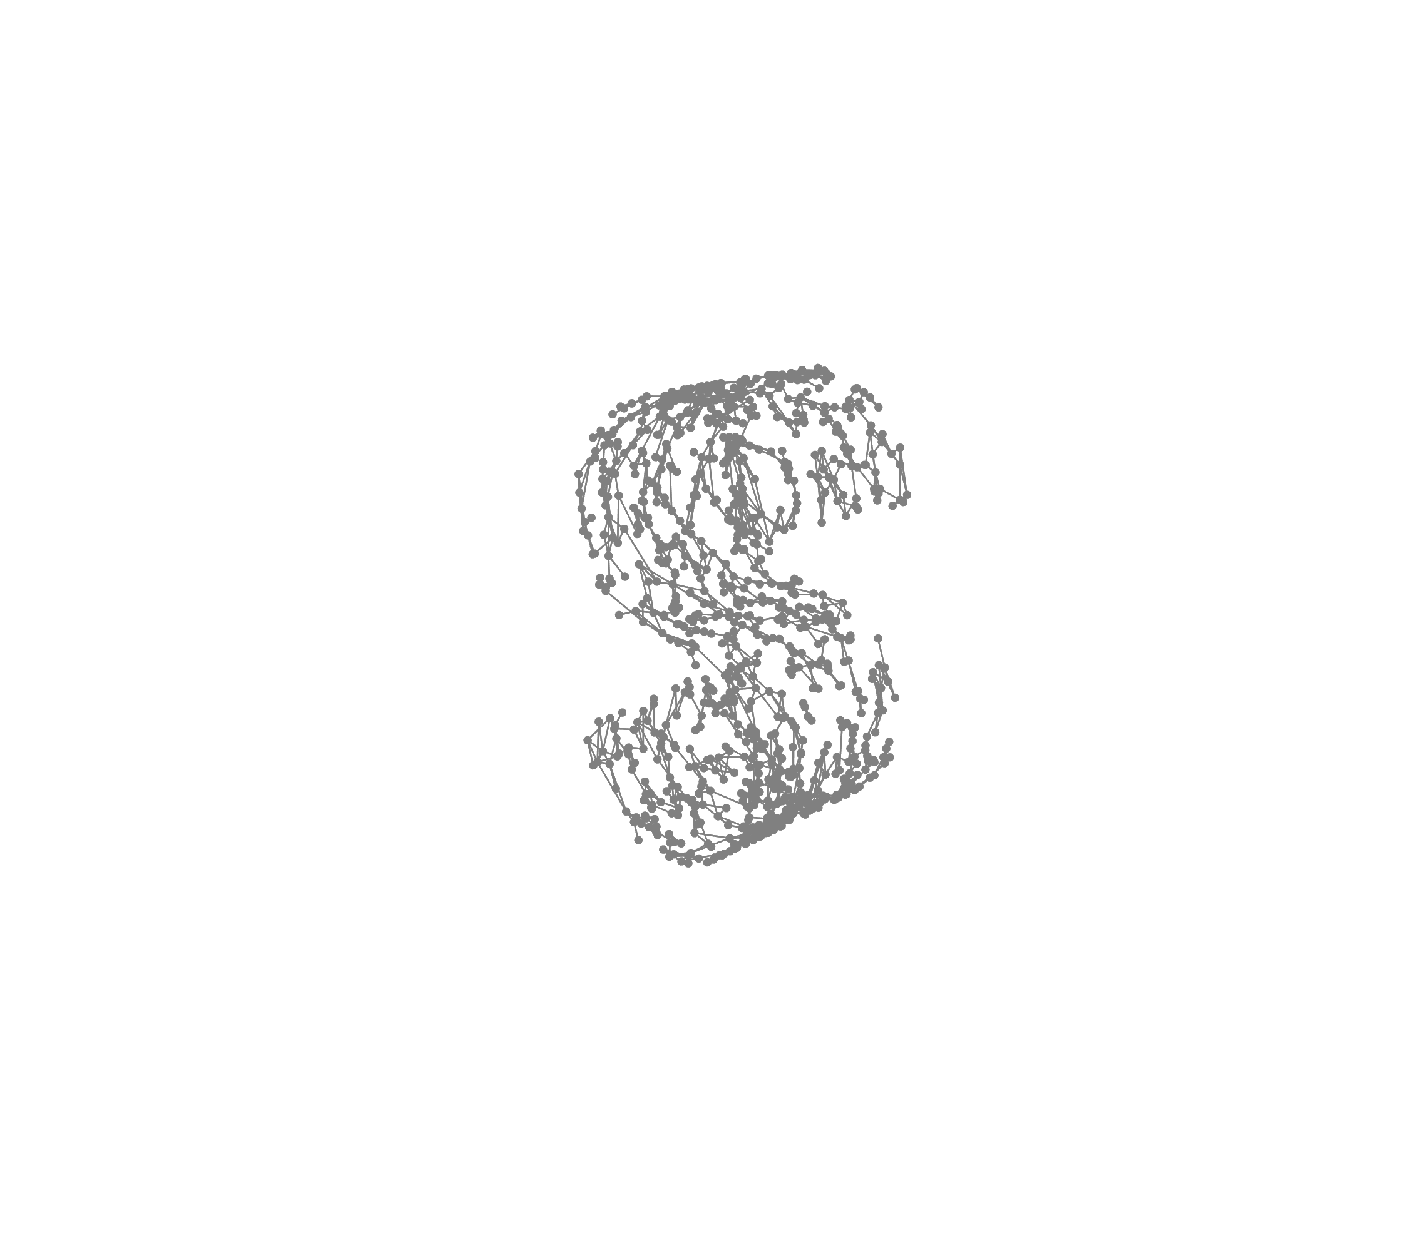
\includegraphics[trim = 250 170 200 140, clip, % left bottom right top
      width = 0.8\textwidth]{figures/s-curve-connected}
    \caption[S-curve neighborhood graph]{$k$-neighborhood graph for 300 points 
    sampled from the S-curve with $k = 3$.
    \textit{Source:} own representation.}
    \label{fig-neighbor-graph}
  \end{figure}
\end{minipage}

% ------------------------------------------------------------------------------

\subsubsection{Eigenanalysis}
\label{eigenanalysis}

Eventually, spectral manifold learning boils down to an eigenanalysis 
of the matrix $\M$ believed to hold information about the intrinsic 
manifold structure.
As explained in chapter \ref{principles-overview}, PCA finds the principal 
eigenvectors of empirical covariance, thereby defining a low-dimensional 
subspace containing most of the data-inherent variability.
The very same idea applies when diagonalizing the more general matrix 
corresponding to the non-linear feature map: the top (or bottom\footnote{
This differs across methods and shall be made clear later.
}) $d$ eigenvectors of $M$ span a subspace into which the data may be projected 
under minimal loss of information.
More precisely, the representation of $\X$ by the $d$ selected eigenvectors of 
$M$ is loss-optimal with respect to the least-squares error
\citep{schoelkopfetal1998}.
Figure \ref{fig:eigen} depicts the idea of eigenanalysis in a schematic way.

\begin{figure}[H]
    \centering
    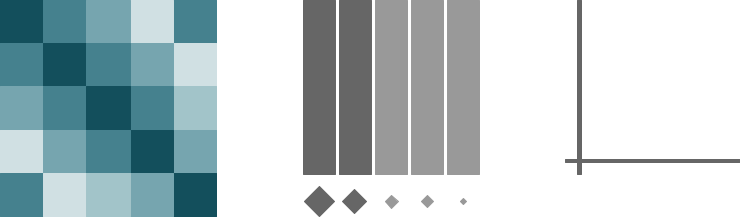
\includegraphics[trim = 0 0 0 0, clip, % left bottom right top
      width = 0.6\textwidth]{figures/eigenanalysis}
    \caption[Schematic view on eigenanalysis]{Conceptual idea of eigenanalysis. 
    Eigenvectors of a matrix (\textit{left}) point in the direction of greatest 
    variability (\textit{middle}), the degree of which is measured by the 
    associated eigenvalues depicted as rhombi. Retaining the thus determined 
    principal $d$ eigenvectors allows to span a linear subspace of reduced 
    dimensionality (\textit{right}).
    \textit{Source:} own representation.}
    \label{fig-eigen}
  \end{figure}

\textbf{Eigenvectors and eigenvalues.} Formally, eigenanalysis is the 
decomposition of a square matrix into pairs of \textit{eigenvectors} and 
\textit{eigenvalues}.
Let $\bm{A} \in \R^{N \times N}$ be a square matrix and $\lambda \in \R$ a 
scalar value. 
$\lambda$ is said to be an eigenvalue to $\bm{A}$ if there exists 
$\bm{v} \in \R^N \setminus \{0\}$ such that $\bm{A} \bm{v} = \lambda \bm{v}$.
Then, $\bm{v}$ is the eigenvector corresponding to the eigenvalue $\lambda$, and 
their tuple is also called an \textit{eigenpair}.
\\

\textbf{Null spaces.} A closely related notion is that of the 
\textit{null space}, consisting of the vectors that map $\bm{A}$ to 0 upon 
multiplication from the right: $\{\bm{v} \in \R^N: \bm{A} \bm{v} = 0\}$.
It can be easily seen that the null space consists of those eigenvectors of 
$\bm{A}$ that are associated with an eigenvalue of zero, and the zero vector 
itself. 
For a specific eigenvalue $\lambda$ of $\bm{A}$, the null space of 
$\lambda \I - \bm{A}$ 
(with $\I$ the $N$-dimensional identity matrix) constitutes the 
\textit{eigenspace} of $\bm{A}$ \citep{boermmehl2012}.
\\

\textbf{Generalized eigenvalue problems.} Eigendecomposition of a matrix 
$\bm{A}$ can be framed as the solution of a generalized eigenvalue problem.
Generalized eigenvalue problems are posed subject to a constraint on a second, 
also symmetric matrix $\bm{B} \in \R^{N \times N}$.
As the standard eigenvalue problem results immediately from 
$\bm{B} = \I$, the generalized form subsumes both cases.
It is given by 

\begin{equation}
  \bm{A} \bm{V} = \bm{B} \bm{V} \bm{\Lambda},
  \label{eq-gevproblem}
\end{equation}

where $\bm{V} = [\bm{v}_1, \bm{v}_2, ..., \bm{v}_N] \in \R^{N \times N}$ 
is the matrix of eigenvectors of $A$ and 
$\bm{\Lambda} = \text{\textit{diag}}[\lambda_1, \lambda_2, ..., \lambda_N]^T 
\in \R^{N \times N}$ is the diagonal matrix of the associated eigenvalues 
(ordered from smallest to largest).
The generalized eigenvalue problem may be stated equivalently as 

\begin{equation}
  \min_{\bm{V}} \text{\textit{trace}}(\bm{V}^T \bm{A} \bm{V}), \quad \text{s.t.} 
  \quad \bm{V}^T \bm{B} \bm{V} = \I,
  \label{eq-gevproblem-max}
\end{equation}

and translated to the first form by means of a Lagrangian multiplier \citep{ghojoghetal2019}.
It must be noted that solving eigenvalue problems becomes computationally 
challenging rather quickly, an issue on which chapter \ref{challenges} 
also briefly comments with regard to the methods discussed here 
\citep{boermmehl2012}.
\\

Building upon the concepts of neighborhood graph approximation and subsequent 
eigenanalysis, the following chapter will now present in detail how LEM, LLE and 
HLLE approach the manifold learning task, and, eventually, how SSLLE seeks to 
improve the low-dimensional embedding through anchoring with prior points.
